% =====================================================================
%  BÁO CÁO PHÂN TÍCH THIẾT KẾ HỆ THỐNG
%  Hệ thống quản lý bất động sản cho thuê (SaaS)
%  Biên dịch bằng XeLaTeX:
%      xelatex -interaction=nonstopmode BAOCAO_DFD.tex
% =====================================================================
\documentclass[12pt,a4paper]{report}

% ---------- Preamble ----------
\usepackage[a4paper,top=2.5cm,bottom=2.5cm,left=3cm,right=2cm]{geometry}
\usepackage{fontspec}
\setmainfont{Times New Roman}
\setsansfont{Arial}

\usepackage{graphicx}
\usepackage{float}
\usepackage{caption}
\usepackage{subcaption}
\usepackage{booktabs}
\usepackage{array}
\usepackage{longtable}
\usepackage{xcolor}
\usepackage{enumitem}
\usepackage{titlesec}
\usepackage{fancyhdr}
\usepackage{setspace}
\usepackage{hyperref}
\hypersetup{colorlinks=true,linkcolor=blue!60!black,urlcolor=blue!60!black}

% ---------- Tiếng Việt không cần gói babel; tăng khả năng co giãn dòng ----------
\tolerance=2000
\emergencystretch=3em
\hyphenpenalty=10000

% ---------- Đặt tên thành phần tiếng Việt ----------
\renewcommand{\contentsname}{Mục lục}
\renewcommand{\chaptername}{Chương}
\renewcommand{\appendixname}{Phụ lục}
\renewcommand{\figurename}{Hình}
\renewcommand{\tablename}{Bảng}
\renewcommand{\listfigurename}{Danh mục hình vẽ}
\renewcommand{\listtablename}{Danh mục bảng}

% ---------- Định dạng tiêu đề ----------
\titleformat{\chapter}[display]
  {\normalfont\huge\bfseries}
  {\chaptertitlename\ \thechapter}
  {12pt}
  {\Huge}
\titlespacing*{\chapter}{0pt}{-20pt}{20pt}

% ---------- Đầu trang / chân trang ----------
\pagestyle{fancy}
\fancyhf{}
\fancyhead[L]{\small\itshape Hệ thống quản lý bất động sản cho thuê}
\fancyhead[R]{\small\itshape Báo cáo Phân tích thiết kế hệ thống}
\fancyfoot[C]{\thepage}
\renewcommand{\headrulewidth}{0.4pt}

% ---------- Khung hình ảnh trống (thiếu ảnh) ----------
% Dùng cho các sơ đồ chưa có ảnh minh họa — để trống theo yêu cầu.
\newcommand{\missingfig}[2][3.5cm]{%
  \begin{figure}[H]
    \centering
    \fbox{%
      \begin{minipage}[c][#1][c]{0.9\textwidth}%
        \vspace{0pt}%
      \end{minipage}}%
    \caption{#2}
  \end{figure}%
}

\setlength{\parindent}{0.6cm}
\linespread{1.3}

% =====================================================================
\begin{document}

% ---------- Trang bìa ----------
\begin{titlepage}
  \begin{center}
    \vspace*{1cm}

    {\LARGE\bfseries BÁO CÁO PHÂN TÍCH THIẾT KẾ HỆ THỐNG}\\[0.6cm]
    {\LARGE\bfseries SƠ ĐỒ LUỒNG DỮ LIỆU (DFD)}\\[1.6cm]

    {\Huge\bfseries HỆ THỐNG QUẢN LÝ}\\[0.2cm]
    {\Huge\bfseries BẤT ĐỘNG SẢN CHO THUÊ}\\[0.2cm]
    {\LARGE\bfseries (SaaS)}\\[2.2cm]

    \rule{0.7\textwidth}{0.8pt}\\[2.4cm]

    \begin{flushleft}
      \hspace{3.5cm}
      \begin{tabular}{@{}ll@{}}
        Nhóm:                 & 8 \\[0.7cm]
        Giảng viên hướng dẫn: & Lê Hữu Thanh Tùng \\[0.7cm]
        Lớp:                  & 012012100802
      \end{tabular}
    \end{flushleft}

    \vfill
    {\large Ngày 11 tháng 8 năm 2026}
  \end{center}
\end{titlepage}

\pagenumbering{roman}
\tableofcontents
\clearpage
\pagenumbering{arabic}

% =====================================================================
% CHƯƠNG 1 — GIỚI THIỆU HỆ THỐNG
% =====================================================================
\chapter{Giới thiệu hệ thống}

\section{Tổng quan về hệ thống}

\textbf{Hệ thống quản lý bất động sản cho thuê} (\emph{Rental Management SaaS}) là một nền tảng phần mềm dưới dạng dịch vụ (Software-as-a-Service) dành cho các chủ nhà trọ, chủ nhà cho thuê và các đơn vị kinh doanh bất động sản cho thuê. Hệ thống giúp số hóa và tự động hóa toàn bộ vòng đời hoạt động cho thuê, bao gồm:

\begin{itemize}[leftmargin=1.2em,itemsep=2pt]
  \item Quản lý tòa nhà, phòng trọ và trạng thái phòng (khả dụng, đang cho thuê, bảo trì);
  \item Quản lý hồ sơ khách thuê, hợp đồng thuê và quy trình kích hoạt tài khoản khách thuê;
  \item Sinh hóa đơn định kỳ theo tháng (tiền phòng, điện, nước, phí khác) và theo dõi tình trạng thanh toán;
  \item Thu thanh toán trực tuyến qua MoMo cùng cơ chế xác nhận tự động (IPN);
  \item Cổng thông tin dành cho khách thuê để tra cứu và thanh toán hóa đơn;
  \item Trợ lý ảo tích hợp trí tuệ nhân tạo (AI Agent) hỗ trợ tra cứu, phân tích và thao tác dữ liệu bằng ngôn ngữ tự nhiên;
  \item Thông báo tự động qua Telegram, email và thông báo trong ứng dụng;
  \item Báo cáo doanh thu, thống kê và xuất file báo cáo (Excel/PDF).
\end{itemize}

\section{Mục tiêu của hệ thống}

\begin{enumerate}[leftmargin=1.6em,itemsep=2pt]
  \item \textbf{Số hóa quy trình:} chuẩn hóa và số hóa toàn bộ quy trình quản lý cho thuê từ tòa nhà, phòng trọ, khách thuê đến hợp đồng và hóa đơn.
  \item \textbf{Tự động hóa:} tự động sinh hóa đơn định kỳ, gửi thông báo nhắc nợ và cảnh báo hết hạn gói dịch vụ.
  \item \textbf{Thanh toán trực tuyến:} hỗ trợ khách thuê và chủ nhà thanh toán trực tuyến qua MoMo với cơ chế xử lý IPN chống trùng lặp.
  \item \textbf{Trải nghiệm khách thuê:} cung cấp cổng thông tin riêng giúp khách thuê tra cứu hóa đơn, lịch sử thanh toán và thanh toán trực tuyến thuận tiện.
  \item \textbf{Trợ lý AI:} hỗ trợ chủ nhà tra cứu dữ liệu (phòng, khách, hợp đồng, doanh thu) và thao tác dữ liệu bằng ngôn ngữ tự nhiên, tiết kiệm thời gian vận hành.
  \item \textbf{Bảo mật:} xác thực bằng JWT (access token + refresh token), OTP qua email, mã hóa dữ liệu nhạy cảm (khóa API thanh toán) và ghi nhật ký kiểm toán (audit log).
\end{enumerate}

\section{Phạm vi của báo cáo}

Báo cáo tập trung phân tích \textbf{luồng dữ liệu (Data Flow Diagram --- DFD)} của toàn bộ hệ thống theo phương pháp phân rã từ trên xuống (top-down): \emph{Sơ đồ ngữ cảnh (Context) → DFD mức 0 → DFD mức 1 → DFD mức 2}, kèm theo mô tả chi tiết từng tiến trình và các kho dữ liệu liên quan, làm cơ sở cho quá trình triển khai và kiểm thử.

\section{Đối tượng sử dụng hệ thống}

\begin{table}[H]
  \centering
  \caption{Các đối tượng sử dụng hệ thống}
  \begin{tabular}{@{}p{3.2cm}p{10.8cm}@{}}
    \toprule
    \textbf{Vai trò} & \textbf{Mô tả} \\
    \midrule
    Chủ nhà (Owner) & Quản lý toàn bộ tòa nhà, phòng trọ, khách thuê, hợp đồng, hóa đơn; đăng ký và nâng cấp gói dịch vụ; sử dụng trợ lý AI; xem báo cáo doanh thu. \textbf{Chủ nhà có thể đồng thời đảm nhận vai trò quản trị viên (Admin)}. \\
    \addlinespace
    Nhân viên (Staff) & Được chủ nhà phân quyền, hỗ trợ các nghiệp vụ vận hành như cập nhật phòng, ghi nhận thanh toán, quản lý khách thuê. \\
    \addlinespace
    Khách thuê (Tenant) & Truy cập cổng thông tin khách thuê, kích hoạt tài khoản, tra cứu hóa đơn và thanh toán trực tuyến qua MoMo. \\
    \addlinespace
    Quản trị viên (Admin) & Vai trò quản trị hệ thống mà \textbf{Chủ nhà có thể đảm nhận}: quản lý gói đăng ký của người dùng, cấu hình cổng thanh toán MoMo, theo dõi thống kê và nhật ký kiểm toán toàn hệ thống. \\
    \bottomrule
  \end{tabular}
\end{table}

\section{Kiến trúc công nghệ dự kiến}

\begin{table}[H]
  \centering
  \caption{Công nghệ và vai trò trong hệ thống}
  \begin{tabular}{@{}p{5.6cm}p{8.4cm}@{}}
    \toprule
    \textbf{Công nghệ} & \textbf{Vai trò} \\
    \midrule
    NestJS (Node.js, TypeScript) & Nền tảng xây dựng REST API backend. \\
    \addlinespace
    MongoDB (Mongoose) & Cơ sở dữ liệu NoSQL, gồm khoảng 20 collection. \\
    \addlinespace
    JWT, OTP qua email & Xác thực người dùng, làm mới phiên (refresh token). \\
    \addlinespace
    MoMo & Cổng thanh toán trực tuyến và xử lý IPN. \\
    \addlinespace
    Telegram Bot API & Kênh thông báo và giao tiếp với người dùng. \\
    \addlinespace
    Resend / SMTP & Gửi email OTP, hợp đồng, hóa đơn và thông báo. \\
    \addlinespace
    OpenAI API (LLM) & Trợ lý AI: sinh câu trả lời và thực thi công cụ (tool). \\
    \addlinespace
    Cloudflare R2 & Lưu trữ file báo cáo xuất ra (Excel/PDF). \\
    \addlinespace
    SSE (Server-Sent Events) & Truyền phát câu trả lời của AI theo thời gian thực. \\
    \bottomrule
  \end{tabular}
\end{table}

\section{Chức năng chính của hệ thống}

Hệ thống gồm \textbf{9 nhóm chức năng chính} tương ứng với 9 tiến trình trong DFD mức 0:

\begin{table}[H]
  \centering
  \caption{Tổng hợp các nhóm chức năng chính}
  \begin{tabular}{@{}c p{4.2cm} p{9cm}@{}}
    \toprule
    \textbf{Mã} & \textbf{Nhóm chức năng} & \textbf{Mô tả} \\
    \midrule
    P1 & Xác thực \& Tài khoản & Đăng ký, đăng nhập, làm mới token, quên/đổi mật khẩu, xác thực email. \\
    \addlinespace
    P2 & Quản lý tòa nhà/Phòng & Quản lý thông tin tòa nhà, phòng trọ, trạng thái phòng. \\
    \addlinespace
    P3 & Khách thuê \& Hợp đồng & Quản lý hồ sơ khách thuê, hợp đồng, kích hoạt khách thuê. \\
    \addlinespace
    P4 & Hóa đơn \& Thanh toán & Sinh hóa đơn định kỳ, ghi nhận thanh toán, tích hợp MoMo. \\
    \addlinespace
    P5 & Gói đăng ký \& Quản trị & Quản lý gói dịch vụ, yêu cầu nâng cấp, quản trị hệ thống. \\
    \addlinespace
    P6 & Cổng thông tin khách thuê & Đăng nhập khách thuê, xem hóa đơn, thanh toán trực tuyến. \\
    \addlinespace
    P7 & AI Agent & Hội thoại, gọi LLM, thực thi tool, theo dõi hạn mức AI. \\
    \addlinespace
    P8 & Báo cáo \& Xuất file & Thống kê doanh thu, xuất báo cáo Excel/PDF lên R2. \\
    \addlinespace
    P9 & Thông báo \& Định kỳ & Gửi thông báo Telegram/email, sinh hóa đơn định kỳ, kiểm toán. \\
    \bottomrule
  \end{tabular}
\end{table}

% =====================================================================
% CHƯƠNG 2 — PHÂN TÍCH DFD
% =====================================================================
\chapter{Phân tích thiết kế luồng dữ liệu (DFD)}

\section{Phương pháp phân tích và ký hiệu sử dụng}

Luồng dữ liệu của hệ thống được phân tích theo quy ước \textbf{Gane-Sarson} với phương pháp phân rã từ trên xuống gồm bốn mức:

\begin{itemize}[leftmargin=1.2em,itemsep=2pt]
  \item \textbf{Mức Context (Sơ đồ ngữ cảnh):} toàn bộ hệ thống được biểu diễn như một tiến trình duy nhất, trao đổi dữ liệu với các thực thể bên ngoài.
  \item \textbf{Mức 0:} phân rã hệ thống thành các tiến trình chính và xác định các kho dữ liệu.
  \item \textbf{Mức 1:} chi tiết hóa các luồng dữ liệu quan trọng của từng tiến trình.
  \item \textbf{Mức 2:} chi tiết hóa tiếp các luồng con cho các nghiệp vụ phức tạp.
\end{itemize}

Các ký hiệu được sử dụng trong sơ đồ được trình bày trong Bảng~\ref{tab:notation}:

\begin{table}[H]
  \centering
  \caption{Ký hiệu sử dụng trong DFD}
  \label{tab:notation}
  \begin{tabular}{@{}p{4.2cm}p{5cm}p{4.8cm}@{}}
    \toprule
    \textbf{Ký hiệu} & \textbf{Ý nghĩa} & \textbf{Ghi chú} \\
    \midrule
    Hình tròn & Tiến trình xử lý (Process) & Một chức năng xử lý dữ liệu \\
    \addlinespace
    Hình chữ nhật & Thực thể ngoài (External Entity) & Người dùng / hệ thống bên ngoài \\
    \addlinespace
    Hình trụ & Kho dữ liệu (Data Store) & Collection trong MongoDB \\
    \addlinespace
    Mũi tên một chiều & Dòng dữ liệu (Data Flow) & Nhãn là danh từ chỉ dữ liệu truyền đi \\
    \bottomrule
  \end{tabular}
\end{table}

Theo đúng chuẩn, tên của \emph{tiến trình} được đặt là động từ (ví dụ: ``Xác thực \& Tài khoản''), còn tên của \emph{dòng dữ liệu} được đặt là danh từ (ví dụ: ``Token truy cập'', ``Hóa đơn'').

\section{Sơ đồ ngữ cảnh (Context Diagram)}

Sơ đồ ngữ cảnh biểu diễn toàn bộ hệ thống như một tiến trình duy nhất, giao tiếp với \textbf{10 thực thể ngoài}:

\begin{itemize}[leftmargin=1.2em,itemsep=2pt]
  \item \textbf{Người dùng:} Chủ nhà (Owner), Nhân viên (Staff), Khách thuê (Tenant), Quản trị viên (Admin). Lưu ý: \emph{Chủ nhà có thể đồng thời đảm nhận vai trò quản trị viên} để quản lý gói dịch vụ, cấu hình thanh toán và xem nhật ký hệ thống.
  \item \textbf{Hệ thống thanh toán:} MoMo.
  \item \textbf{Hệ thống truyền thông:} Telegram Bot, Email/SMTP.
  \item \textbf{Hệ thống bên ngoài khác:} OpenAI LLM, Cloudflare R2.
\end{itemize}

Các luồng dữ liệu chính tại mức này:

\begin{itemize}[leftmargin=1.2em,itemsep=2pt]
  \item \emph{Người dùng → Hệ thống:} thông tin đăng nhập, dữ liệu tòa nhà/phòng/khách/hóa đơn, yêu cầu thanh toán, câu hỏi AI.
  \item \emph{Hệ thống → Người dùng:} token truy cập, hợp đồng, hóa đơn, xác nhận thanh toán, thống kê.
  \item \emph{Hệ thống → MoMo:} yêu cầu tạo thanh toán; nhận về URL thanh toán và thông báo IPN.
  \item \emph{Hệ thống → Telegram/Email:} tin nhắn thông báo, email xác thực/OTP/hợp đồng/hóa đơn.
  \item \emph{Hệ thống → OpenAI:} prompt và lời gọi công cụ; nhận phản hồi LLM.
  \item \emph{Hệ thống → Cloudflare R2:} lưu trữ file báo cáo Excel/PDF; đọc lại file khi cần.
\end{itemize}

Sơ đồ ngữ cảnh được thể hiện trong Hình~\ref{fig:context}:

\begin{figure}[H]
  \centering
  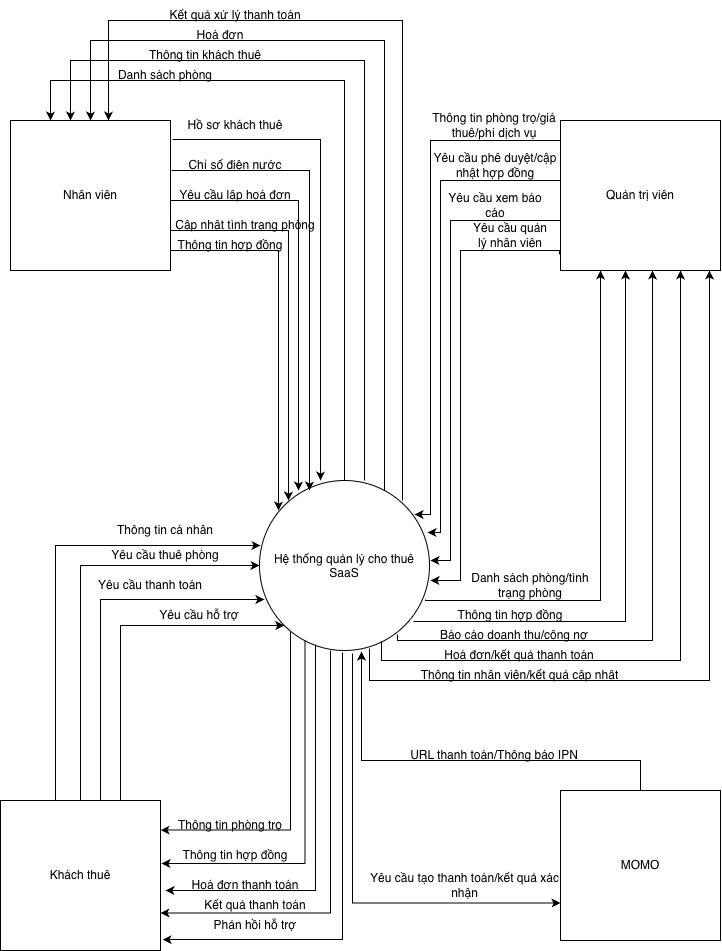
\includegraphics[width=0.82\textwidth,keepaspectratio]{images/context/context.jpg}
  \caption{Sơ đồ ngữ cảnh (Context Diagram) của hệ thống}
  \label{fig:context}
\end{figure}

\section{DFD mức 0 --- Phân rã các tiến trình chính}

Tại mức 0, hệ thống được phân rã thành \textbf{9 tiến trình chính} (P1 -- P9), giao tiếp với \textbf{10 thực thể ngoài} và đọc/ghi trên \textbf{15 kho dữ liệu} (collection MongoDB). Chi tiết từng tiến trình được trình bày ở Bảng~\ref{tab:process0}.

\begin{table}[H]
  \centering
  \caption{Danh sách tiến trình tại DFD mức 0}
  \label{tab:process0}
  \begin{tabular}{@{}c p{4.4cm} p{8.6cm}@{}}
    \toprule
    \textbf{Mã} & \textbf{Tiến trình} & \textbf{Vai trò} \\
    \midrule
    P1 & Xác thực \& Tài khoản & Xử lý đăng ký, đăng nhập, token, OTP, xác thực email. \\
    P2 & Quản lý tòa nhà / Phòng & Quản lý tòa nhà, phòng trọ và trạng thái phòng. \\
    P3 & Khách thuê \& Hợp đồng & Quản lý hồ sơ khách thuê, hợp đồng, kích hoạt tài khoản. \\
    P4 & Hóa đơn \& Thanh toán & Sinh hóa đơn, ghi nhận thanh toán, tích hợp cổng thanh toán. \\
    P5 & Gói đăng ký \& Quản trị & Quản lý gói dịch vụ, nâng cấp gói, quản trị hệ thống. \\
    P6 & Cổng thông tin khách thuê & Cung cấp giao diện cho khách thuê tra cứu, thanh toán. \\
    P7 & AI Agent & Hội thoại, gọi LLM, thực thi công cụ, theo dõi hạn mức. \\
    P8 & Báo cáo \& Xuất file & Tổng hợp số liệu và xuất báo cáo Excel/PDF. \\
    P9 & Thông báo \& Định kỳ & Gửi thông báo Telegram/email, sinh hóa đơn định kỳ, ghi audit. \\
    \bottomrule
  \end{tabular}
\end{table}

\textbf{Các kho dữ liệu} được sử dụng tại mức 0 gồm: \texttt{USERS}, \texttt{AUTH} (refresh token), \texttt{OTPS}, \texttt{PROPERTIES}, \texttt{ROOMS}, \texttt{TENANTS}, \texttt{CONTRACTS}, \texttt{BILLS}, \texttt{PAYMENTS}, \texttt{PAYSETTINGS}, \texttt{SUBSCRIPTIONS}, \texttt{UPGRADES}, \texttt{NOTIFS}, \texttt{AUDIT}, \texttt{AI DATA}.

\textbf{Các luồng dữ liệu quan trọng} tại mức 0:

\begin{itemize}[leftmargin=1.2em,itemsep=2pt]
  \item Chủ nhà gửi dữ liệu tòa nhà/phòng đến P2; P2 gửi trạng thái phòng (\texttt{OCCUPIED}/\texttt{AVAILABLE}) đến P3.
  \item P4 nhận yêu cầu thanh toán từ P6 (cổng thông tin khách thuê) và gửi kết quả thanh toán ngược lại.
  \item P4 và P7 kiểm tra hạn mức gói tại kho \texttt{SUBSCRIPTIONS} (P5) trước khi thực hiện nghiệp vụ.
  \item P4 trao đổi với MoMo (tạo thanh toán, nhận URL và IPN) để thu tiền hóa đơn; P5 thanh toán gói qua MoMo.
  \item P7 trao đổi với OpenAI (prompt, lời gọi tool, phản hồi LLM); P8 lưu/đọc file trên Cloudflare R2.
  \item P1, P3, P4 yêu cầu P9 gửi email thông báo (OTP, hợp đồng, hóa đơn quá hạn).
\end{itemize}

DFD mức 0 được thể hiện trong Hình~\ref{fig:dfd0}:

\begin{figure}[H]
  \centering
  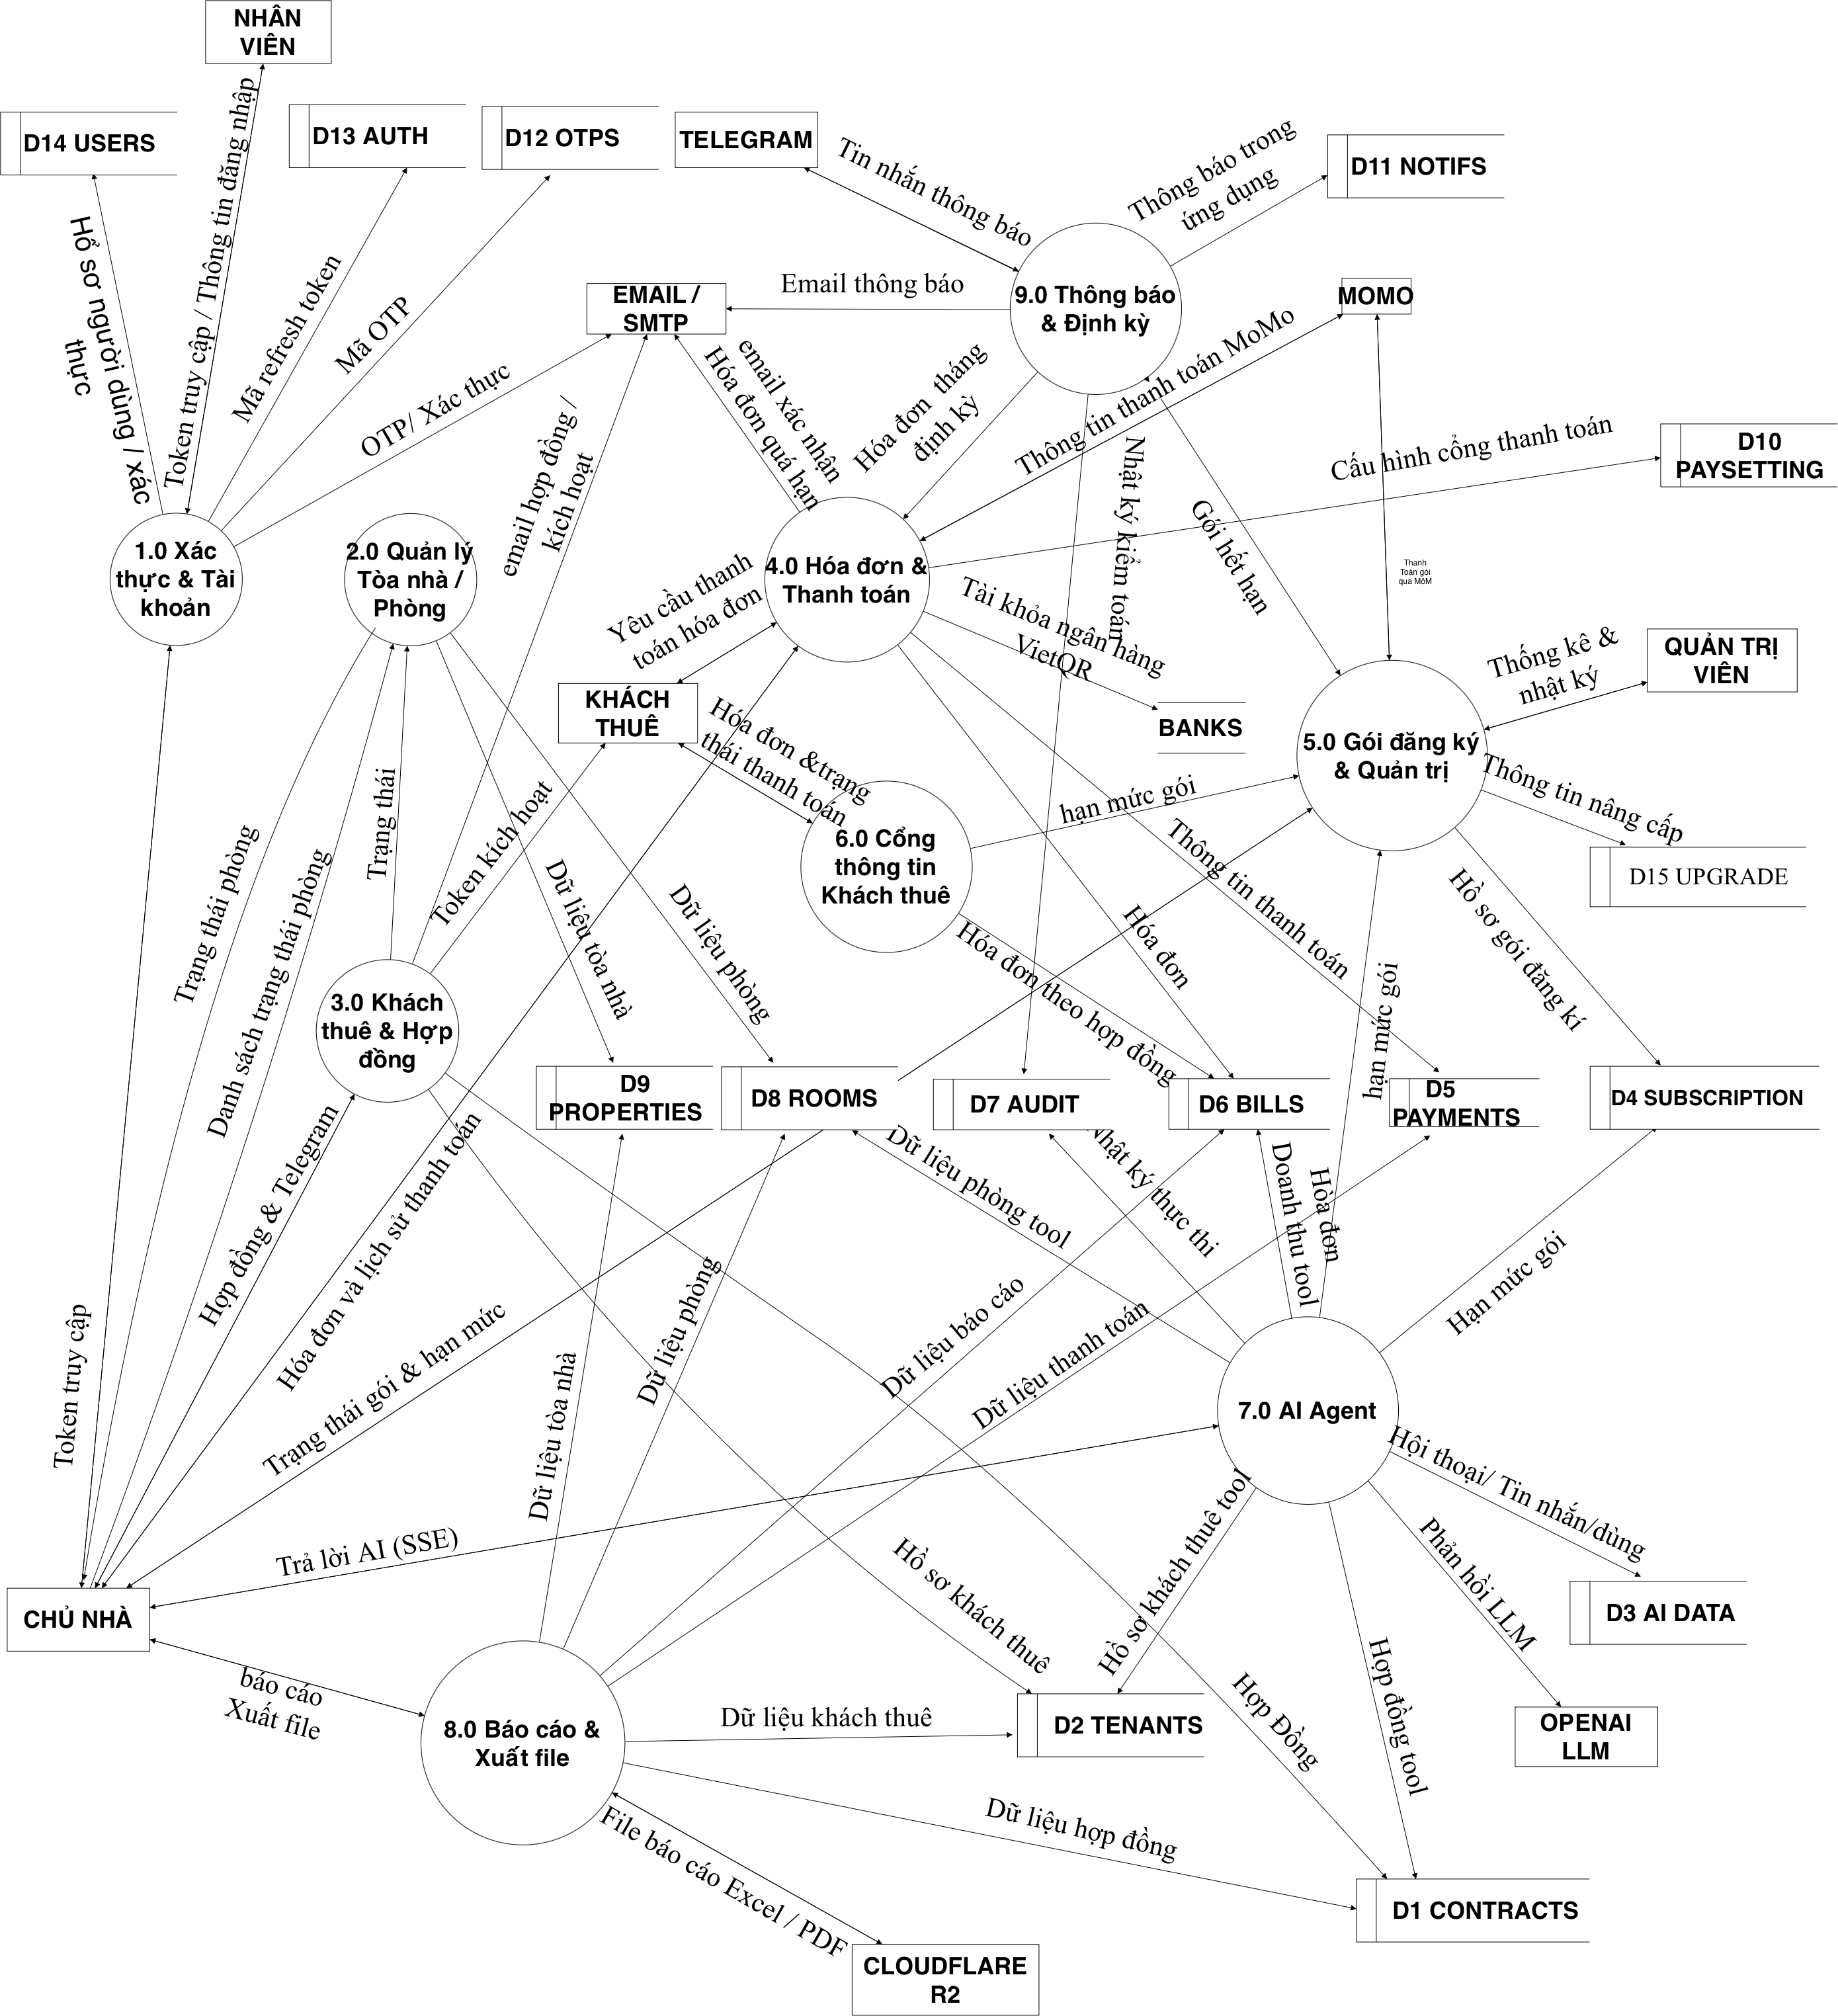
\includegraphics[width=0.82\textwidth,keepaspectratio]{images/level_0/dfd_0-2.png}
  \caption{DFD mức 0 --- Phân rã các tiến trình chính của hệ thống}
  \label{fig:dfd0}
\end{figure}

\section{DFD mức 1 --- Chi tiết các luồng quan trọng}

DFD mức 1 chi tiết hóa \textbf{6 luồng nghiệp vụ quan trọng} của hệ thống, với đầy đủ ảnh minh họa và mô tả chi tiết cho từng luồng.

\subsection{Xác thực \& Tài khoản (P1)}

Tiến trình xác thực bao gồm các nghiệp vụ: \emph{đăng ký} (sinh mã OTP, gửi email, tạo gói FREE/trial), \emph{đăng nhập} (xác minh thông tin, phát hành cặp token), \emph{làm mới token} (dùng refresh token, thu hồi token cũ), \emph{quên/đổi mật khẩu} (OTP qua email, cập nhật mật khẩu đã băm) và \emph{xác thực email}. Các kho dữ liệu liên quan: \texttt{USERS}, \texttt{AUTH}, \texttt{OTPS}, \texttt{SUBSCRIPTIONS}. Thực thể ngoài: Chủ nhà và Email/SMTP. Sơ đồ được thể hiện trong Hình~\ref{fig:dfd11}:

\begin{figure}[H]
  \centering
  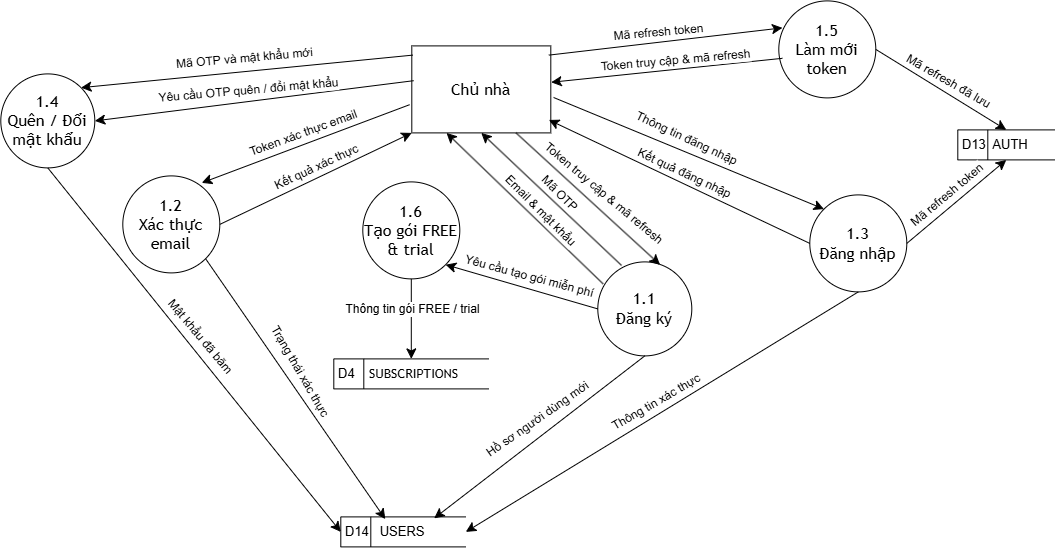
\includegraphics[width=0.9\textwidth,keepaspectratio]{images/level_1/dfd_1_1.png}
  \caption{DFD mức 1 --- Xác thực \& Tài khoản}
  \label{fig:dfd11}
\end{figure}

\subsection{Hợp đồng \& Kích hoạt khách thuê (P3)}

Khi chủ nhà tạo hợp đồng, hệ thống kiểm tra phòng còn khả dụng trong \texttt{ROOMS}, lưu hợp đồng mới (trạng thái \texttt{ACTIVE}) vào \texttt{CONTRACTS}, cập nhật phòng sang \texttt{OCCUPIED} và gửi email kèm \emph{link kích hoạt} cho khách thuê. Khách thuê dùng token kích hoạt để đặt mật khẩu khởi tạo (đánh dấu cờ \texttt{mustChangePassword}); hợp đồng kết thúc sẽ được chuyển sang trạng thái \texttt{TERMINATED} và phòng trở lại \texttt{AVAILABLE}. Sơ đồ được thể hiện trong Hình~\ref{fig:dfd12}:

\begin{figure}[H]
  \centering
  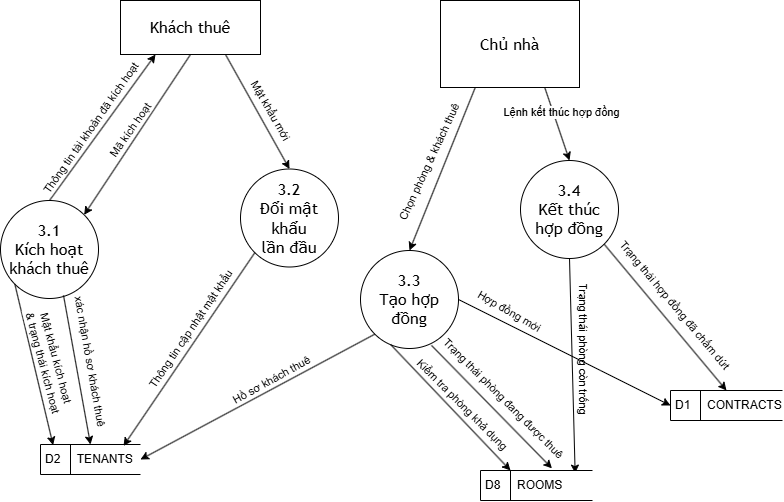
\includegraphics[width=0.75\textwidth,keepaspectratio]{images/level_1/dfd_1_2.png}
  \caption{DFD mức 1 --- Hợp đồng \& Kích hoạt khách thuê}
  \label{fig:dfd12}
\end{figure}

\subsection{Hóa đơn \& Thanh toán (P4)}

Chủ nhà nhập số điện/nước và phí khác; hệ thống tính toán dựa trên giá phòng trong \texttt{CONTRACTS} và sinh hóa đơn tháng trong \texttt{BILLS}. Thanh toán có thể được ghi nhận trực tiếp (tiền mặt/chuyển khoản) hoặc thực hiện trực tuyến qua MoMo. Các thông báo IPN được xử lý tại tiến trình con \emph{Xử lý IPN} với kiểm tra chữ ký và chống trùng giao dịch (\texttt{transactionId}) trước khi cập nhật số tiền đã trả và trạng thái hóa đơn. Sơ đồ được thể hiện trong Hình~\ref{fig:dfd13}:

\begin{figure}[H]
  \centering
  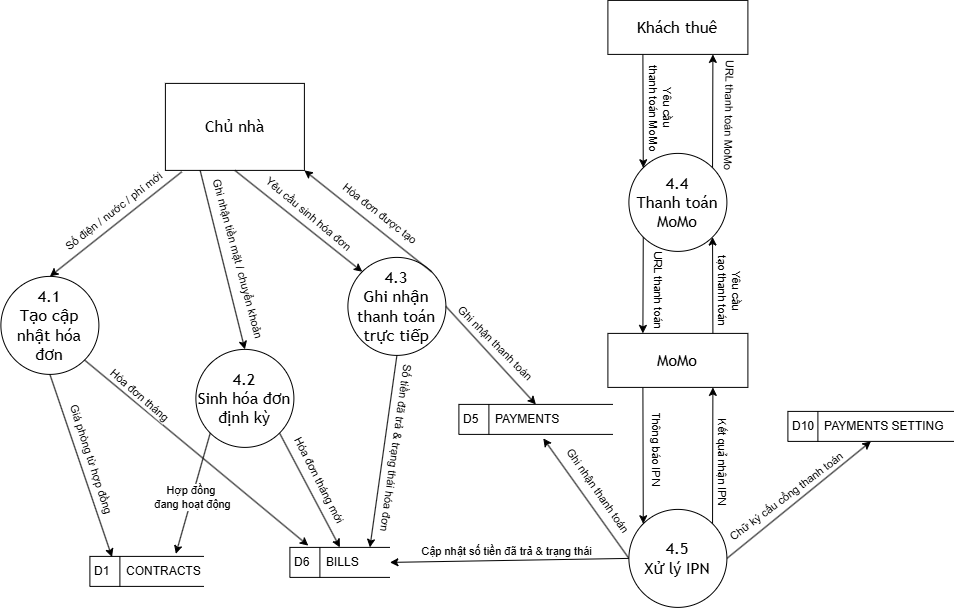
\includegraphics[width=0.8\textwidth,keepaspectratio]{images/level_1/dfd_1_3.png}
  \caption{DFD mức 1 --- Hóa đơn \& Thanh toán}
  \label{fig:dfd13}
\end{figure}

\subsection{Gói đăng ký \& Nâng cấp (P5)}

Hệ thống kiểm tra gói hiện tại và hạn mức (số tòa nhà, phòng, nhân viên) trong \texttt{SUBSCRIPTIONS}, \texttt{PROPERTIES}, \texttt{ROOMS}, \texttt{USERS}. Chủ nhà có thể gửi yêu cầu nâng cấp (lưu vào \texttt{UPGRADES} với trạng thái \texttt{PENDING}) và thanh toán qua MoMo; khi nhận IPN hợp lệ, hệ thống kích hoạt gói mới và cập nhật yêu cầu sang \texttt{APPROVED}. Chủ nhà (đảm nhận vai trò quản trị viên) có thể kích hoạt gói trực tiếp và cấu hình khóa MoMo. Tiến trình định kỳ \emph{hết hạn gói} sẽ hạ cấp về gói FREE. Sơ đồ được thể hiện trong Hình~\ref{fig:dfd14}:

\begin{figure}[H]
  \centering
  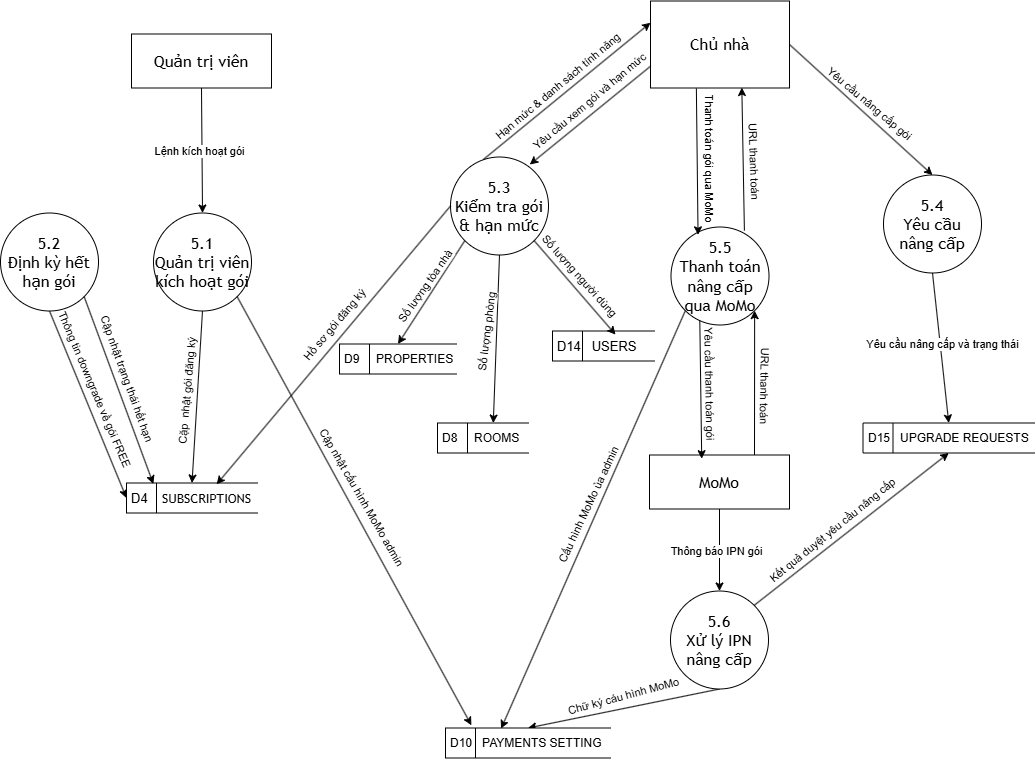
\includegraphics[width=0.8\textwidth,keepaspectratio]{images/level_1/dfd_1_4.png}
  \caption{DFD mức 1 --- Gói đăng ký \& Nâng cấp}
  \label{fig:dfd14}
\end{figure}

\subsection{AI Agent (P7)}

Tiến trình AI Agent gồm: quản lý hội thoại (lưu vào \texttt{AI DATA}), vòng lặp agent (gửi prompt và lời gọi công cụ đến OpenAI, nhận phản hồi LLM), thực thi công cụ (đọc/ghi \texttt{ROOMS}, \texttt{TENANTS}, \texttt{CONTRACTS}, \texttt{BILLS}; ghi nhật ký vào \texttt{AUDIT}) và theo dõi hạn mức AI (\texttt{SUBSCRIPTIONS}, \texttt{AI DATA}). Kết quả được trả về cho chủ nhà theo giao thức SSE theo thời gian thực. Sơ đồ được thể hiện trong Hình~\ref{fig:dfd15}:

\begin{figure}[H]
  \centering
  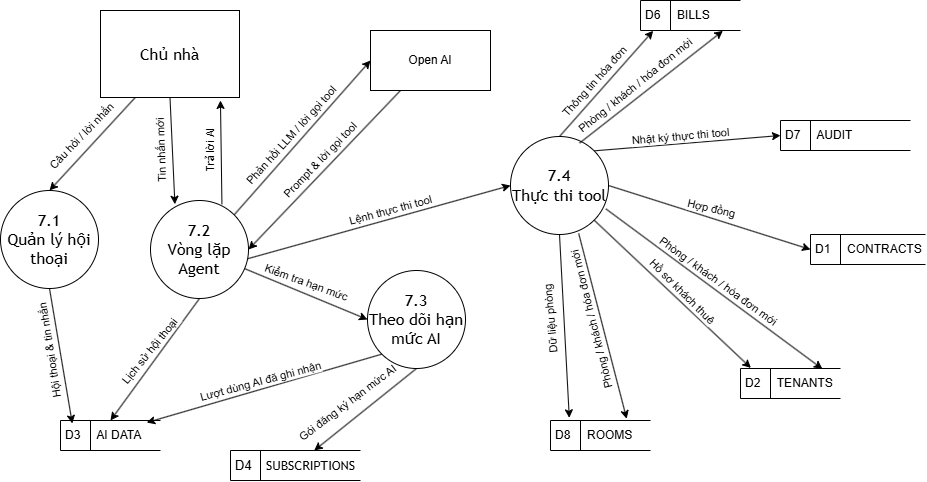
\includegraphics[width=0.8\textwidth,keepaspectratio]{images/level_1/dfd_1_5.png}
  \caption{DFD mức 1 --- AI Agent}
  \label{fig:dfd15}
\end{figure}

\subsection{Cổng thông tin khách thuê (P6)}

Khách thuê đăng nhập vào cổng thông tin (xác minh qua \texttt{TENANTS}), xem danh sách hóa đơn theo hợp đồng (\texttt{CONTRACTS}, \texttt{BILLS}) cùng lịch sử thanh toán (\texttt{PAYMENTS}), sau đó thực hiện thanh toán trực tuyến qua MoMo dựa trên danh sách phương thức thanh toán khả dụng trong \texttt{PAYSETTINGS}. Sơ đồ được thể hiện trong Hình~\ref{fig:dfd16}:

\begin{figure}[H]
  \centering
  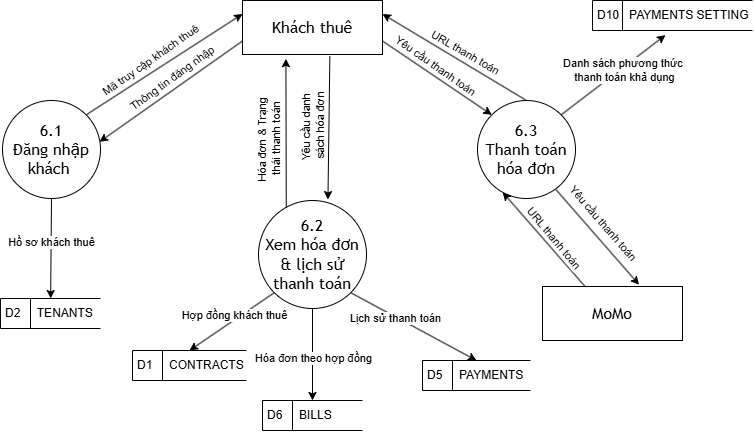
\includegraphics[width=0.7\textwidth,keepaspectratio]{images/level_1/dfd_1_6.png}
  \caption{DFD mức 1 --- Cổng thông tin khách thuê}
  \label{fig:dfd16}
\end{figure}

\section{DFD mức 2 --- Chi tiết các luồng con}

DFD mức 2 chi tiết hóa các luồng con cho những nghiệp vụ phức tạp, gồm \textbf{4 luồng} với đầy đủ ảnh minh họa cho từng luồng.

\subsection{Luồng Đăng ký \& Đăng nhập (OTP + Token)}

Luồng đăng ký bắt đầu khi chủ nhà gửi \emph{email, mật khẩu, họ tên}; tiến trình con \textbf{1.1.1 Nhận yêu cầu đăng ký} lưu mã OTP đăng ký (hiệu lực 5 phút) vào \texttt{OTPS} và gửi email chứa mã OTP. Tại tiến trình con \textbf{1.1.2 Xác minh OTP đăng ký}, khi khách thuê nhập đúng mã, hệ thống xóa mã đã dùng, tạo hồ sơ người dùng mới với trạng thái \texttt{emailVerified} trong \texttt{USERS}, tự động tạo gói FREE/trial 14 ngày trong \texttt{SUBSCRIPTIONS} và trả về cặp token. Luồng đăng nhập xác minh thông tin trong \texttt{USERS}, phát hành refresh token vào \texttt{AUTH} và trả cặp token mới. Luồng làm mới token kiểm tra refresh token còn hạn/chưa thu hồi trong \texttt{AUTH}, thu hồi token cũ và cấp cặp token mới. Sơ đồ được thể hiện trong Hình~\ref{fig:dfd21}:

\begin{figure}[H]
  \centering
  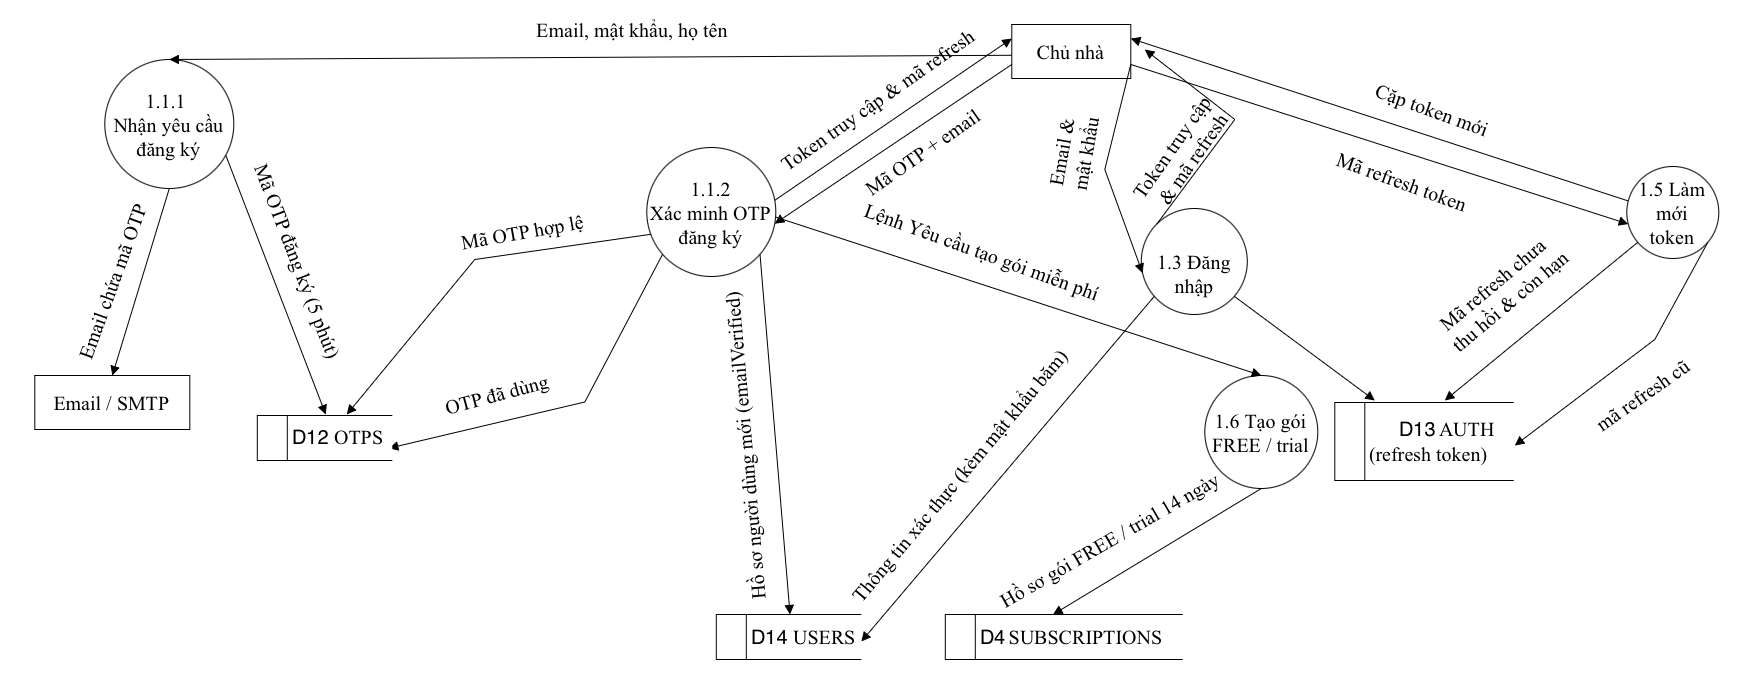
\includegraphics[width=0.95\textwidth,keepaspectratio]{images/level_2/dfd_2_1.png}
  \caption{DFD mức 2 --- Luồng Đăng ký \& Đăng nhập (OTP + Token)}
  \label{fig:dfd21}
\end{figure}

\subsection{Luồng Thanh toán hóa đơn qua MoMo (tạo + IPN)}

Khách thuê gửi yêu cầu thanh toán; tiến trình con \textbf{4.4.1 Tạo yêu cầu thanh toán MoMo} đọc hóa đơn còn nợ trong \texttt{BILLS}, lấy cấu hình MoMo của chủ nhà (giải mã khóa từ \texttt{PAYSETTINGS}) và tạo yêu cầu thanh toán với \texttt{orderId = billId + thời gian} gửi đến MoMo. MoMo trả về \texttt{payUrl/deeplink/QR} để chuyển tiếp cho khách thuê. Khi MoMo gửi IPN (\texttt{orderId, transId, resultCode}), tiến trình \textbf{4.5 Xử lý IPN MoMo} xác minh cấu hình theo \texttt{partnerCode}, kiểm tra trùng \texttt{transId} trong \texttt{PAYMENTS}, ghi nhận giao dịch, cập nhật số tiền đã trả và trạng thái hóa đơn trong \texttt{BILLS}, sau đó phản hồi kết quả xác nhận cho MoMo. Sơ đồ được thể hiện trong Hình~\ref{fig:dfd22}:

\begin{figure}[H]
  \centering
  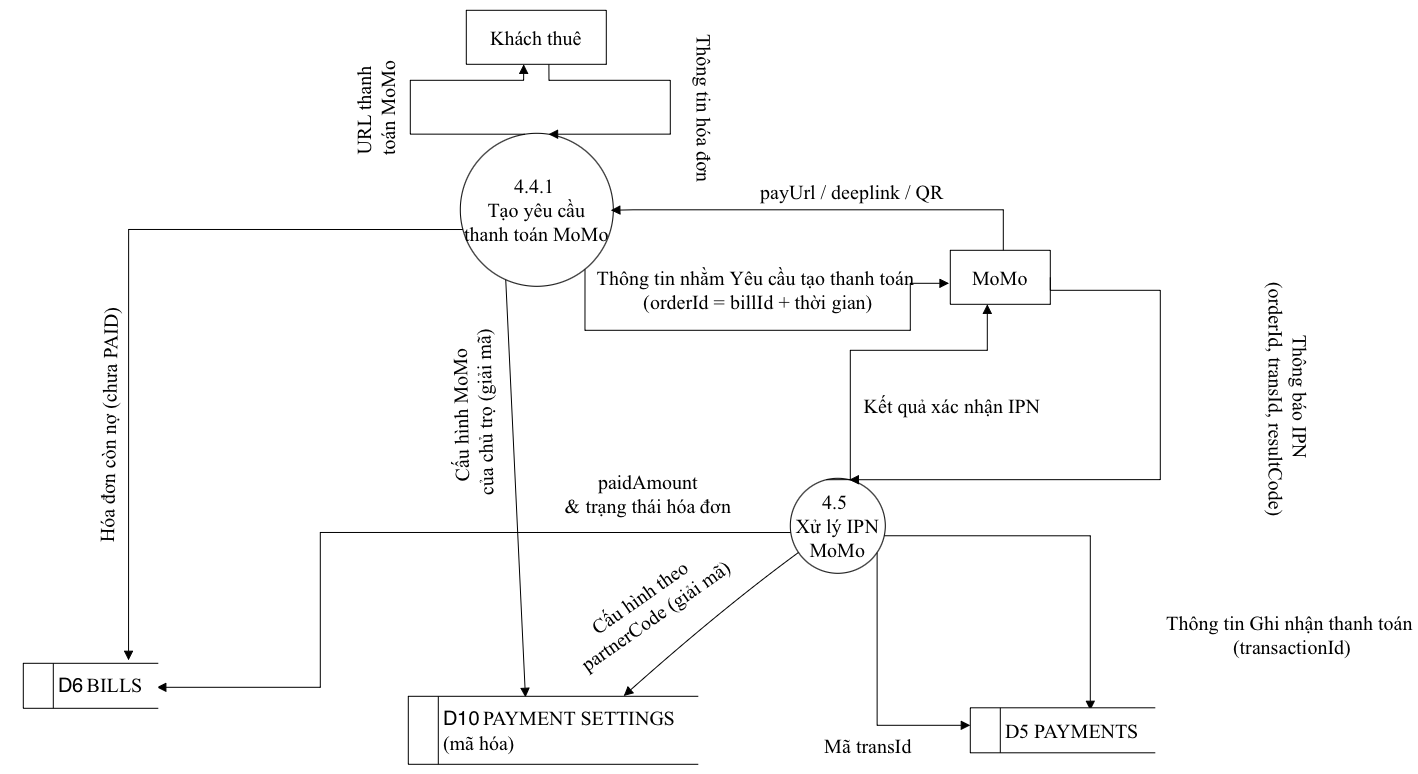
\includegraphics[width=0.9\textwidth,keepaspectratio]{images/level_2/dfd_2_2.png}
  \caption{DFD mức 2 --- Luồng Thanh toán hóa đơn qua MoMo (tạo + IPN)}
  \label{fig:dfd22}
\end{figure}

\subsection{Luồng Nâng cấp gói qua MoMo (tạo + IPN)}

Chủ nhà gửi yêu cầu nâng cấp (\texttt{plan}, \texttt{months}); tiến trình con \textbf{5.5.1 Tạo thanh toán nâng cấp gói} đọc giá và gói hiện tại trong \texttt{SUBSCRIPTIONS}, lấy cấu hình MoMo của quản trị viên từ \texttt{PAYSETTINGS} (giải mã khóa), tạo yêu cầu thanh toán (\texttt{orderId} chứa thông tin gói, chủ nhà và số tháng) và lưu yêu cầu nâng cấp trạng thái \texttt{PENDING} vào \texttt{UPGRADES}. Khi nhận IPN gói, tiến trình \textbf{5.6 Xử lý IPN nâng cấp gói} xác minh chữ ký theo cấu hình admin, sau đó tiến trình con \textbf{5.1.1 Kích hoạt gói} cập nhật gói mới trong \texttt{SUBSCRIPTIONS} và chuyển yêu cầu sang \texttt{APPROVED}. Sơ đồ được thể hiện trong Hình~\ref{fig:dfd24}:

\begin{figure}[H]
  \centering
  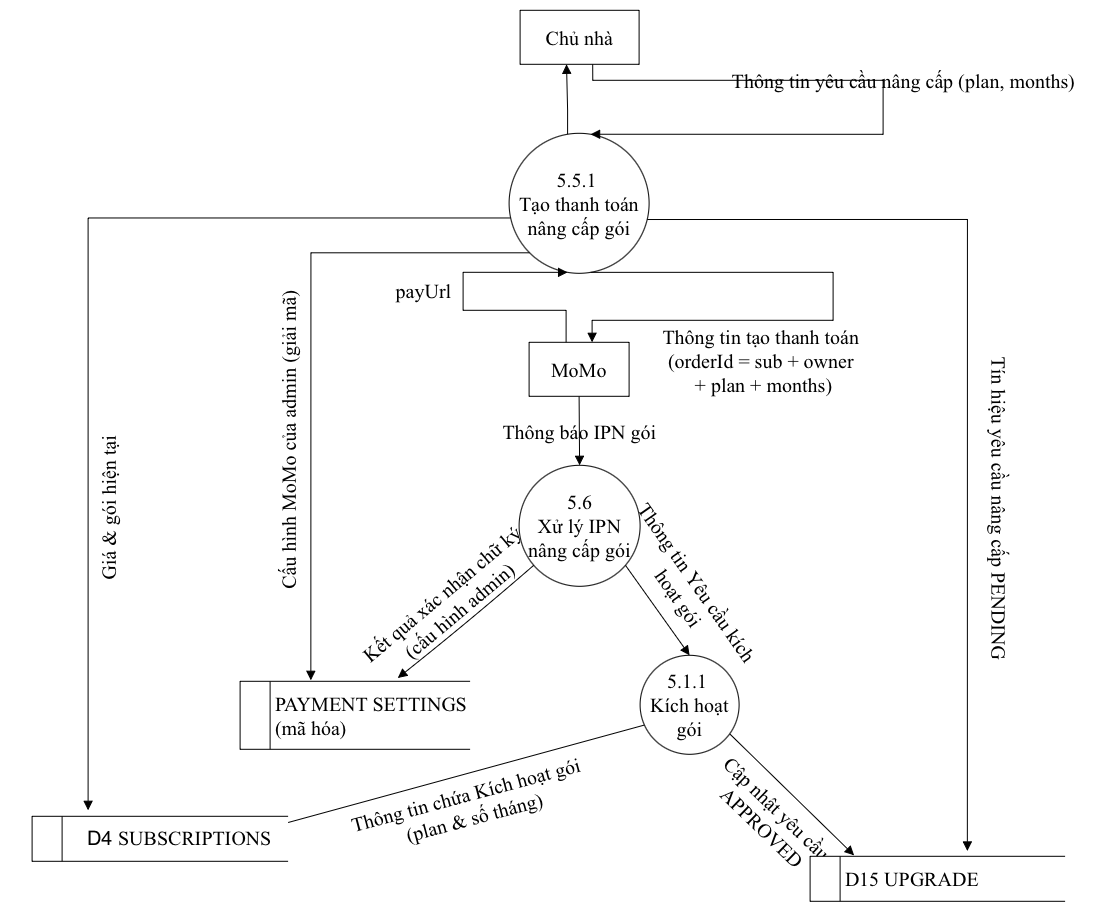
\includegraphics[width=0.85\textwidth,keepaspectratio]{images/level_2/dfd_2_4.png}
  \caption{DFD mức 2 --- Luồng Nâng cấp gói qua MoMo (tạo + IPN)}
  \label{fig:dfd24}
\end{figure}

\subsection{Vòng lặp AI Agent \& Thực thi công cụ}

Vòng lặp AI Agent bắt đầu khi chủ nhà gửi tin nhắn mới: tiến trình con \textbf{7.2.1 Phân tích yêu cầu} kiểm tra hạn mức gói trong \texttt{SUBSCRIPTIONS} và lưu tin nhắn cùng lịch sử hội thoại vào \texttt{AI DATA}; tiến trình con \textbf{7.2.2 Gọi LLM} xây dựng prompt và gửi đến OpenAI. Nếu LLM yêu cầu thực thi công cụ, tiến trình con \textbf{7.2.3 Thực thi tool} đọc/ghi trên \texttt{ROOMS}, \texttt{TENANTS}, \texttt{CONTRACTS}, \texttt{BILLS}, ghi nhật ký vào \texttt{AUDIT} và đưa kết quả công cụ trở lại vòng lặp để LLM tiếp tục. Cuối cùng, tiến trình con \textbf{7.3.1 Ghi nhận lượt dùng} lưu câu trả lời vào \texttt{AI DATA}, ghi nhận lượt dùng AI và trả về cho chủ nhà qua SSE. Sơ đồ được thể hiện trong Hình~\ref{fig:dfd25}:

\begin{figure}[H]
  \centering
  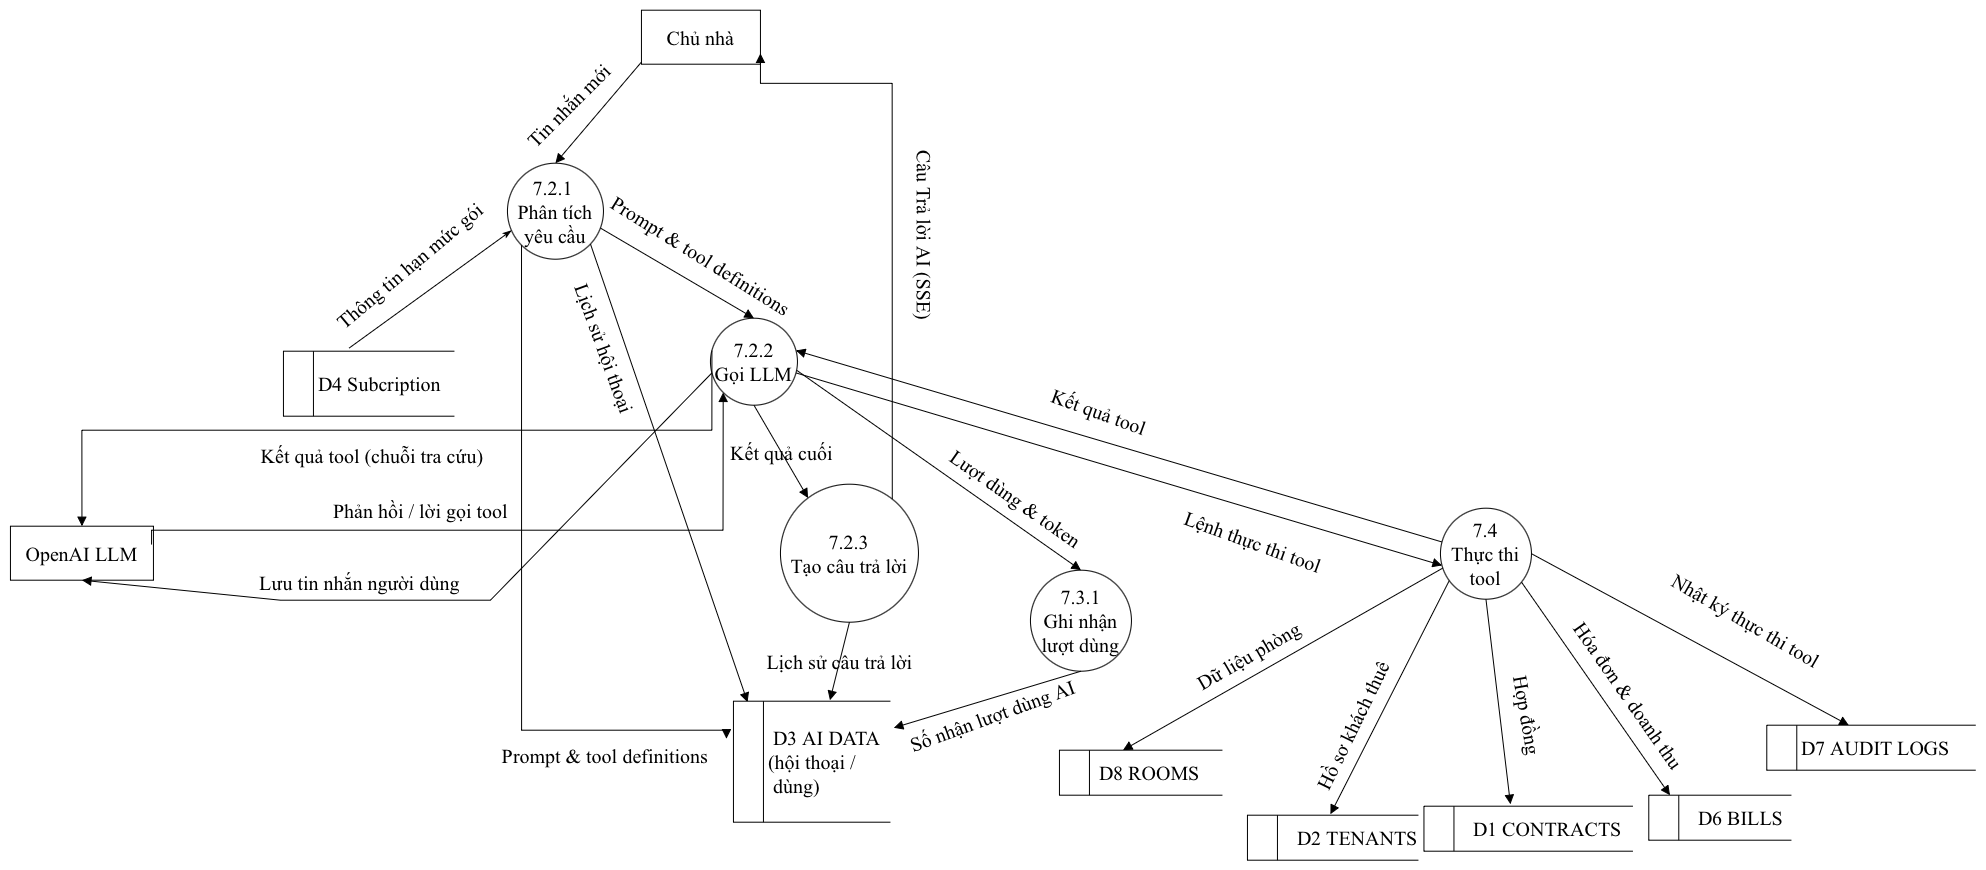
\includegraphics[width=0.9\textwidth,keepaspectratio]{images/level_2/dfd2_5.png}
  \caption{DFD mức 2 --- Vòng lặp AI Agent \& Thực thi công cụ}
  \label{fig:dfd25}
\end{figure}

\end{document}
